%%%%%%%%%%%%%%%%%%%%%%%%%%%%%%%%%%%%%%%%%
% Two Column Curriculum Vitae XeLaTeX Template
%
% This template has been downloaded from:
% http://www.latextemplates.com
%
% Original author:
% Alessandro (The CV Inn)
%
% IMPORTANT: THIS TEMPLATE NEEDS TO BE COMPILED WITH XeLaTeX
%
% This template uses several fonts not included with Windows/Linux by
% default. If you get compilation errors saying a font is missing, find the line
% on which the font is used and either change it to a font included with your
% operating system or comment the line out to use the default font.
% 
%%%%%%%%%%%%%%%%%%%%%%%%%%%%%%%%%%%%%%%%%

%%%%%%%%%%
% General notes:
%
% Font face can be temporarily changed with \fontspec{Family_name}.
%%%%%%%%%%

%----------------------------------------------------------------------------------------
%	PACKAGES AND OTHER DOCUMENT CONFIGURATIONS
%----------------------------------------------------------------------------------------

\documentclass[10pt]{article} % Font size (10pt, 11pt or 12pt)

\usepackage[hmargin=1cm, vmargin=1cm]{geometry} % Document margins
\usepackage{amsmath}
\usepackage{marvosym} % Required for symbols in the colored box
\usepackage{ifsym} % Required for symbols in the colored box
\usepackage[usenames,dvipsnames]{xcolor} % Allows the definition of hex colors

% Fonts and tweaks for XeLaTeX
\usepackage{fontspec,xltxtra,xunicode}
\defaultfontfeatures{Mapping=tex-text}
\setromanfont[Mapping=tex-text]{Palatino Linotype} % Main document font
\setsansfont[Scale=MatchLowercase,Mapping=tex-text]{Calibri} % Font for your name at the top
%\setmonofont[Scale=MatchLowercase]{Consolas}

% Colors for links, text and headings
\usepackage{hyperref}
\definecolor{linkcolor}{HTML}{66391A} % Links  
\definecolor{shade}{HTML}{F5DD9D} % Peach color for the contact information box
\definecolor{text1}{HTML}{2b2b2b} % Main document font color, off-black
\definecolor{headings}{HTML}{393085} % Headings
%\definecolor{faint}{HTML}{777777} % De-emphasis colour
% Other color palettes: shade=B9D7D9 and linkcolor=A40000; shade=D4D7FE and linkcolor=FF0080

\hypersetup{colorlinks,breaklinks, urlcolor=linkcolor, linkcolor=linkcolor} % Set up links and colors

\usepackage{fancyhdr}
\pagestyle{fancy}
\fancyhf{}
\rfoot{\color{text1} \today}
% Headers and footers can be added with the \lhead{} \rhead{} \lfoot{} \rfoot{} commands
% Example footer:
%\rfoot{\color{headings} {\sffamily Last update: \today}. Typeset with Xe\LaTeX}

% Positions the footer in the correct place - number is measured from the top
% (edge? margin end?) of the page
\setlength{\textheight}{24.25cm}

\renewcommand{\headrulewidth}{0pt} % Get rid of the default rule in the header

\usepackage{titlesec} % Allows creating custom \section's

% Format of the section titles
\titleformat{\section}{\color{headings}\fontspec{HelveticaNeue LT 63 MdEx}
\scshape\normalsize\raggedright}{}{0em}{}[\color{black}\titlerule]

\titlespacing{\section}{0pt}{0pt}{0pt} % Spacing around titles


\begin{document}

\color{text1} % Sets the default text color for the whole document

%
%
%	NAME
%
%

\begin{minipage}[t]{0.5\textwidth}
\vspace{0pt} % Trick for alignment

\vspace*{1em}
\par{\centering{\sffamily\fontsize{36pt}{30pt}\selectfont William Berg}\\}
\par{\centering{\color{headings}Software engineer\\}}
\vspace*{\fill}

\end{minipage} % End left-hand side of the page
\begin{minipage}[t]{0.44\textwidth} 
\vspace{0pt} %trick for alignment

%
%
%   CONTACT DETAILS
%
%

\colorbox{shade}{\textcolor{text1}{
\begin{tabular}{c|p{7cm}}
\raisebox{-3pt}{\textifsymbol{18}} & 12 Friars Pl Ln, London, UK W3 7AW \\ % Address 
%\raisebox{-3pt}{\Mobilefone} & +44 (0)7951 491 360 \\ % Phone number
\raisebox{-2pt}{\Letter} & \href{mailto:william.berg08@gmail.com}{william.berg08@gmail.com} \\ % Email address
\raisebox{-1pt}{\Keyboard} & \href{http://wberg.mine.nu}{http://wberg.mine.nu} \\ % Website

\includegraphics[width=10pt]{res/external_link} &
\href{http://uk.linkedin.com/pub/william-berg/27/309/72a}{
\includegraphics[height=10pt]{res/linkedin}}
\href{http://stackoverflow.com/users/1047597/william-berg}{
\includegraphics[height=10pt]{res/stackoverflow}} % yes, these have to be pdfs or the links won't work. flatex
\href{http://careers.stackoverflow.com/wberg}{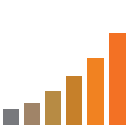
\includegraphics[height=10pt]{res/stackoverflow_careers}}
\end{tabular}
}}\\[10pt]
	
\end{minipage} % End right-hand side of the page

%
%
%   MAIN CONTENT
%
%

%----------------------------------------------------------------------------------------
%	EDUCATION
%----------------------------------------------------------------------------------------

%\section{\fontsize{11pt}{101pt}\selectfont Education} 
\section{Education}
\hfill \break

\begin{tabular}{l l l}

2008 -- 2012 & \textbf{MEng (Hons) Computing (2:1)} & \textit{Imperial College London}\\
2002 -- 2008 & \textbf{A-level} & \textit{Latymer Upper School}\\

\end{tabular}\\[10pt]

%----------------------------------------------------------------------------------------
%	EXPERIENCE
%----------------------------------------------------------------------------------------

\section{Experience}
\hfill \break

\begin{tabular}{l p{0.8\linewidth}}

2014 -- 2015 & \textbf{Software engineer} at \textit{MetaBroadcast} \\
& I worked part-time at MetaBroadcast whilst simultaneously developing an Android app that enhanced phone functionality in real-time by analysing contextual audio from the microphone. I later stopped development on the app and joined full time, working mainly with Java. Continuous integration was managed with Jenkins. Projects I worked on include: \\
& \parbox{0.8\textwidth}{
  \begin{itemize}
  \item An application that took school curricula and supplied metadata for relevant educational video clips for a client's application
  \item A system that managed a cache of suggested content for a programme recommendation service
  \end{itemize}}
&
2012 -- 2014 & \textbf{Software engineer} at \textit{OpenMarket} \\
& I worked in the Solutions Consulting team. I worked with team members and clients to specify, develop and maintain a range of Java web applications that managed customer subscriptions and performed mass-mailing for clients. We used custom tools to achieve continuous integration. Projects I worked on included: \\
& \parbox{0.8\textwidth}{
  \begin{itemize}
  \setlength\itemsep{-1em}
  \item A system that allowed charity organisers to automatically deliver content to users in return for donations \\
  \item Web applications that managed promotional subscriptions for mobile phone company users \\
  \item A company-internal file storage system using Apache Cassandra for metadata \\
  \end{itemize}}
&
2011 \textit{($\frac{1}{2}$ yr)} & \textbf{Software development internship} at \textit{Amadeus} \\
& I wrote a prototype for the Baggage Reconciliation System, a mobile Windows Forms app in C\#. I integrated with the back-end with C++.\\

\end{tabular}\\[10pt]

%----------------------------------------------------------------------------------------
%	OTHER SOFTWARE
%----------------------------------------------------------------------------------------

\section{Other software}
\hfill \break

\begin{tabular}{l l}

Ask me about \textit{drumman}, \textit{ListenerApp}, \textit{TimTom} and other personal projects available on \href{http://github.com/williamberg}{GitHub 
\includegraphics[height=1em]{res/github}} /williamberg & \\
 & \\

\end{tabular}\\[10pt]

%----------------------------------------------------------------------------------------
%	MEMBERSHIPS AND HOBBIES
%----------------------------------------------------------------------------------------

\section{Memberships and hobbies}
\hfill \break

\href{http://www.meiquan.co.uk/}{
\includegraphics[height=2em]{res/tai_chi_symbol}} Mei Quan Taiji
\hspace{3em}
\href{https://soundcloud.com/dj_niceberg/}{\includegraphics[height=2em]{res/soundcloud}} /dj\_niceberg
\\[10pt]

%----------------------------------------------------------------------------------------
%	CERTIFICATION
%----------------------------------------------------------------------------------------

\section{Certification}
\hfill \break

\begin{tabular}{l l}

UK driver & \\
Grade 5 ABRSM piano and music theory

\end{tabular}\\[10pt]

\end{document}  
